\documentclass[12pt]{beamer}
\usetheme{Singapore}
\usepackage{mathpazo}
\renewcommand{\rmdefault}{ppl}
\setbeamerfont{title}{family=\rmfamily}
\setbeamerfont{frametitle}{family=\rmfamily}
\usepackage[utf8]{inputenc}
\usefonttheme{professionalfonts} 
\usepackage{amsmath}
\usepackage{amsfonts}
\usepackage{amssymb}
\usepackage{xcolor}
\usepackage{listings}
\usepackage{tikz}
\usetikzlibrary{positioning,fit}

\author{Lai Hao Ran \\ \footnotesize\texttt{hrlai.ecology@gmail.com}}
\title{Understanding random effects as priors}
\date{} 
%\setbeamercovered{transparent} 
\setbeamertemplate{navigation symbols}{} 

\titlegraphic{%
	\centering
	
\includegraphics[height=0.15\textheight]{fig/Marsden-logo-RGB-150.jpg}~%
	\hspace{1cm}
	
\includegraphics[height=0.15\textheight]{fig/University_of_Canterbury_logo.png}~%
	\hspace{1cm}
	
\includegraphics[height=0.15\textheight]{fig/searpp.png}
} 

\newcommand{\exercise}{%
  \begin{tikzpicture}[remember picture, overlay]
    \node[anchor=north east] at (current page.north east) {
        
\includegraphics[width=2.5cm]{fig/exercise.png}
    };
  \end{tikzpicture}%
}

\begin{document}

\begin{frame}
\titlepage
\end{frame}

\begin{frame}{What is a prior?}
\begin{center}
To put it simply:

\bigskip

\begin{tikzpicture}[
roundnode/.style={circle, draw, thick, minimum width=2cm, align=center},
rectnode/.style={rectangle, draw, thick, minimum width=2cm, minimum height=1cm, align=center},
]
%Nodes
\node[roundnode] (post) {Posterior};
\node[rectnode] (mod) [right=1cm of post] {Model};
\node (input) [right=1cm of mod] {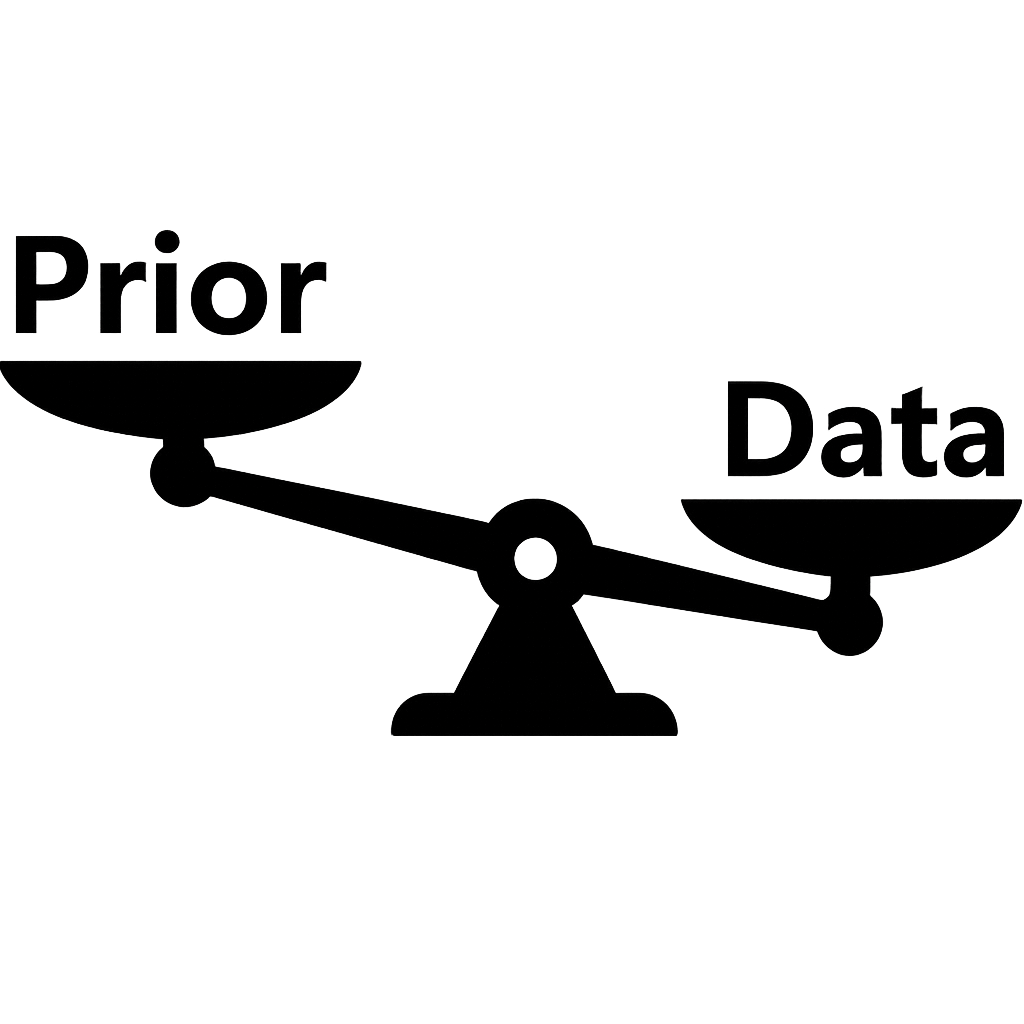
\includegraphics[width=3cm]{fig/data-prior.png}};
%Lines
\draw[-stealth, very thick] (mod) -- (post);
\draw[-stealth, very thick] (input) -- (mod);
\end{tikzpicture}
\end{center}
\end{frame}

\begin{frame}{Our mathematical model, in full}
\begin{align*}
Y &\sim \text{Normal}(\mu, \sigma_\epsilon) \\
\mu &= \alpha + \beta X \\
\alpha &\sim \text{Normal}(0, 10) \\
\beta &\sim \text{Normal}(0, 10) \\
\sigma_\epsilon &\sim \text{Normal}^{+}(0, 10) \\
\end{align*}
\vfill
\alert{
Whiteboard:
\begin{enumerate}
\item Draw prior distributions
\item Update it with strong and weak data
\end{enumerate}
}
\end{frame}

\begin{frame}{Five levels of priors}
\begin{table}
\begin{tabular}{ll}
\hline
Prior type & Example \\
\hline
Flat & $\text{Normal}(0, \infty)$ \\
Super-vague but proper & $\text{Normal}(0, 10^6)$ \\
Weakly informative & $\text{Normal}(0, 10)$ \\
Generic weakly informative & $\text{Normal}(0, 1)$ \\
Informative & $\text{Normal}(-0.47, 0.15)$ \\
\hline
\end{tabular}
\end{table}
\begin{center}
\alert{Whiteboard: overlay priors}
\end{center}
\end{frame}

\begin{frame}{Prior guessing}
\exercise
\begin{columns}
\begin{column}{0.45\textwidth}
\uncover<1->{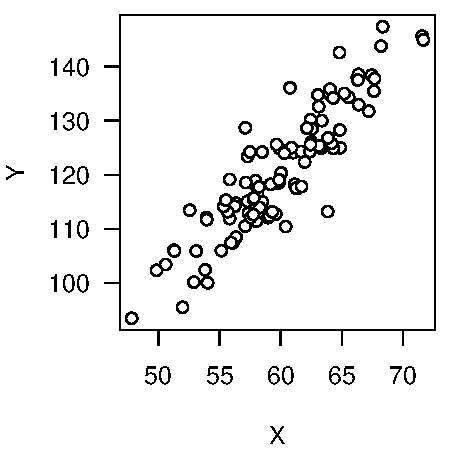
\includegraphics[width=\textwidth]{fig/prior-guess1.pdf}} %
\end{column}
\begin{column}{0.45\textwidth}
\uncover<2->{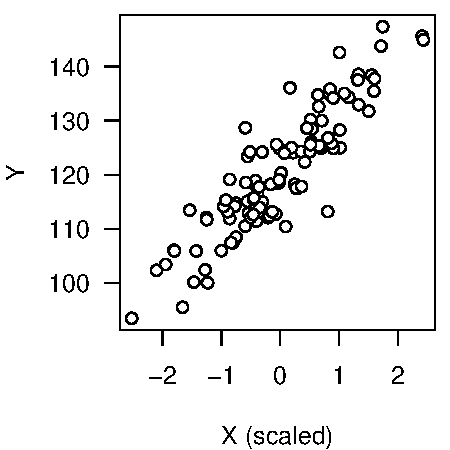
\includegraphics[width=\textwidth]{fig/prior-guess2.pdf}} %
\end{column}
\end{columns}
\uncover<3>{
\begin{center}
Prior choice depends on the data scale!
\end{center}
}
\end{frame}

\begin{frame}{Detour: on subjectivity}
\begin{itemize}[<+->]
\item Model choice is as subjective as prior choice
\item Leaving the prior as flat is as subjective as making it weakly informative
\item Think of ``subjectivity'' as ``transparency''
\end{itemize}
\end{frame}

\begin{frame}[t]{From fixed to random effects:\\it's in the priors}
\only<1>{
\begin{align*}
Y &\sim \text{Normal}(\mu, \sigma_\epsilon) \\
\mu &= \alpha + \beta X \\
\alpha &\sim \text{Normal}(0, 10) \\
\beta &\sim \text{Normal}(0, 10) \\
\sigma_\epsilon &\sim \text{Normal}^{+}(0, 10) \\
\end{align*}
}
\only<2>{
\begin{align*}
Y &\sim \text{Normal}(\mu, \sigma_\epsilon) \\
\mu &= \alpha + \beta X \\
\alpha &\sim \text{Normal}(0, \textcolor{blue}{\sigma_\alpha}) \\
\beta &\sim \text{Normal}(0, \textcolor{blue}{\sigma_\beta}) \\
\sigma_\epsilon &\sim \text{Normal}^{+}(0, 10) \\
\end{align*}
}
\only<3>{
\begin{align*}
Y &\sim \text{Normal}(\mu, \sigma_\epsilon) \\
\mu &= \alpha + \beta X \\
\alpha &\sim \text{Normal}(0, \textcolor{blue}{\sigma_\alpha}) \\
\beta &\sim \text{Normal}(0, \textcolor{blue}{\sigma_\beta}) \\
\sigma_\epsilon &\sim \text{Normal}^{+}(0, 10) \\
\textcolor{blue}{\sigma_\alpha} & \textcolor{blue}{ \sim \text{Normal}^{+}(0, 10) } \\
\textcolor{blue}{\sigma_\beta} & \textcolor{blue}{ \sim \text{Normal}^{+}(0, 10) } \\
\end{align*}
}
\end{frame}

\end{document}